

\documentclass{beamer}
 
\usepackage[utf8]{inputenc}
\usetheme{CambridgeUS}
\useinnertheme{circles}

\usefonttheme[onlymath]{serif} 
 
%Information to be included in the title page:

\title{Seminar 1}
\subtitle{Overview of modern physics}

\author{Will Barker\inst{1}\inst{2}}
\institute{
  \inst{1}%
    Cavendish Laboratory\\
    University of Cambridge\\
  \inst{2}%
    Kavli Institute for Cosmology\\
    University of Cambridge\\
}
\date{}
\logo{%
  \makebox[0.95\paperwidth]{%
    
\includegraphics[height=0.7cm,keepaspectratio]{CU.eps}%
    \hfill%
    \includegraphics[height=0.7cm,keepaspectratio]{logo.png}%
  }%
}
 
 
 
\begin{document}
 
\frame{\titlepage}
 
\begin{frame}
\frametitle{Scope of `\textit{Physics \& Astronomy: Week 1}'}
\begin{itemize}
  \item<1-> Seminar 1: Overview of modern physics
  \item<2-> Seminar 2: Overview of Astrophysics
  \item<3-> Seminar 3: Calculus and classical mechanics
  \item<4-> Seminar 4: Special relativity
  \item<5-> Seminar 5: General relativity
\end{itemize}
\end{frame}

\begin{frame}
  \frametitle{What is physics?}
  \begin{itemize}
    \item<1-> Space?
    \item<2-> Time?
    \item<3-> Energy?
    \item<4-> Forces?
    \item<5-> \textbf{Mathematical description of all these things}
  \end{itemize}
\end{frame}

\begin{frame}
  \frametitle{What is physics?}
  \begin{itemize}
    \item<1-> \textit{a priori} (thermodynamics, statistical physics)
    \item<2-> \textit{a posteriori} (almost everything else!)
    \item<3-> This breakdown of physical laws is often not a clean one\ldots
  \end{itemize}
\end{frame}

\begin{frame}
\frametitle{Branches of physics by history}
\begin{itemize}
  \item<1-> We've been concocting physical laws for thousands of years
  \item<2-> Ancient: strongly representative of everyday world
  \item<3-> Modern: weakly representative of everyday world
\end{itemize}
\end{frame}

\begin{frame}
\frametitle{Branches of physics by history}
\begin{itemize}
  \item<1-> Ancient Greece:
    \begin{itemize}
      \item<2-> 500-700 BCE: Pre-Socratic philosophers (Thales, Anaximenes, Anaximander) express physical laws concerning magnets, electrostatically charged amber, and posit cosmologies
      \item<3-> 400-500 BCE: Leucippus and Democritus posit atomic theory with absolutely no evidence, this clashes with Parmenides' view of a continuous universe -- both are upheld by modern physics
      \item<4-> 300-400 BCE: Aristotle proposes sweeping physical theories based on four `elements' of earth, fire, air and water -- this does lasting damage up to and including the times of Newton
      \item<5-> 200-300 BCE: Eratosthenes calculates the Earth's radius, Plutarch and Seleucus posit heliocentrism, Archimedes lays foundations of static mechanics and hydrodynamics
      \item<6-> 100-200 BCE: Hipparchus makes contributions to astronomy and predicts eclipses
    \end{itemize}
\end{itemize}
\end{frame}

\begin{frame}
\frametitle{Branches of physics by history}
\begin{itemize}
  \item<1-> Ancient India:
    \begin{itemize}
      \item<2-> 400-500 BCE: Aryabhata posits Earths's rotation
      \item<3-> 200-300 BCE: Maharishi Kanada independently develops atomic theory, however this appears to be ingrained in the Buddhist tradition from 600 BCE through to the first millenium -- again there is no evidence
      \item<4-> 1400-1600 CE: Somayaji posits heliocentrism
    \end{itemize}
  \item<5-> Ancient China:
    \begin{itemize}
      \item<6-> 400-500 BCE: Kuo works on genuine magnetism and optics, developing the pinhole camera
    \end{itemize}
\end{itemize}
\end{frame}

\begin{frame}
\frametitle{Branches of physics by history}
\begin{itemize}
  \item<1-> Medieval Islamic world:
    \begin{itemize}
      \item<2-> 700-1500 CE: Aristotelian and Ptolemaic physics is translated into Arabic
      \item<3-> 900-1000 CE: Al-Haytham establishes optics and the r\^ole of light in vision, along with the scientific method, meanwhile Avicenna develops some good ideas about mechanics (i.e. qualitative version of Newton's laws)
      \item<4-> 1000-1100 CE: Abu'l-Barakat finalises Newton's 2nd law, while Ibn Bajjah provides Newton's 3rd law
      \item<5-> 1200-1300 CE: Al-Tusi and his students once again arrive at heliocentrism, so far even as elliptical orbits
    \end{itemize}
  \item<6-> Medieval Europe:
    \begin{itemize}
      \item<7-> So far as I can tell, discovered very little\ldots
    \end{itemize}
\end{itemize}
\end{frame}

\begin{frame}
\frametitle{Branches of physics by history}
\begin{itemize}
  \item<1-> Renaissance Europe:
    \begin{itemize}
      \item<2-> 1400-1600 CE: Copernicus, Brahe develop modern heliocentrism, Kepler adds his three laws of planetary motion, Galileo studies the pendulum and classical gravity, and discovers the Galilean moons
      \item<3-> 1600-1800 CE: Descartes gives us Cartesian coordinates, Leibniz and Newton develop calculus, Newton finally develops his three laws of motion along with the corpuscular theory of light, Newton's law of cooling, speed of sound and Newtonian gravity -- this was reconciled with Kepler's laws; meanwhile Boyle, Hooke Gay-Lussac, Papin, Watt and others develop certain thermodynamic principles (though they aren't integrated)
    \end{itemize}
\end{itemize}
\end{frame}

\begin{frame}
\frametitle{Branches of physics by history}
\begin{itemize}
  \item<1-> 18th century Europe:
    \begin{itemize}
      \item<2-> Bernoulli develops hydrodynamics
      \item<3-> Cavendish measures $G$
      \item<4-> Herschel discovers Uranus
      \item<5-> Michell suggests classical black holes
      \item<6-> Euler, Legendre, d'Alembert, Laplace and Lagrange begin general application of mathematical methods to mechanics
    \end{itemize}
\end{itemize}
\end{frame}

\begin{frame}
\frametitle{Branches of physics by history}
\begin{itemize}
  \item<1-> 19th century Europe:
    \begin{itemize}
      \item<2-> Faraday, Weber, Hertz and Gauss make contributions to early electromagnetism, Maxwell concludes this with the Maxwell equations
      \item<3-> Kelvin, Clausius, Helmholtz, Carnot, Joule Boltzmann, Gibbs and Maxwell converge on statistical mechanics, based on previous thermodynamic laws
      \item<4-> R\"ontgen, Becquerel, Curie and Rutherford discover spontaneous radiation
    \end{itemize}
\end{itemize}
\end{frame}

\begin{frame}
\frametitle{Branches of physics by history}
\begin{itemize}
  \item<1-> 20th century world:
    \begin{itemize}
      \item<2-> Einstein, in response to questions raised by Michelson, Morley, Maxwell and others, proposes special relativity
      \item<3-> Planck, Einstein, Bohr, de Broglie, Compton, Pauli, Dirac, Fermi, Bose, Born and Heisenberg develop the old quantum theory in response to a myriad of inconsistencies within classical mechanics and statistical physics, quantum mechanics evolves from this
      \item<4-> Einstein, building on mathematics developed by Riemann, Lorentz, Cartan and others, proposes general relativity
      \item<5-> Dirac, Feynman, Schwinger, Gell-Mann, Weinberg, Yang, Mills, Higgs and others merge special relativity and quantum mechanics to produce quantum field theory, gauge field theory and the standard model
    \end{itemize}
\end{itemize}
\end{frame}

\begin{frame}
\frametitle{Branches of physics by regime}
\begin{itemize}
  \item<1-> Can split the field up according to \textbf{regimes}
  \item<2-> Different physical laws apply to the same situation, but only become true when the variables are sufficiently large, small, or comprable to certain \textbf{fundamental constants}
  \item<3-> Kinetic energy (relativistic regime): $T\equiv mc^2\left(1/\sqrt{1-v^2/c^2}-1\right)$
  \item<4-> Kinetic energy (non-relativistic regime): $T\approx mv^2/2$
  \item<5-> Seldom representative of the everyday world
\end{itemize}
\end{frame}

\begin{frame}
  \frametitle{Regimes in graphics}
\center
\includegraphics[height=3cm]{Classical-and-modern-physics.png}
\includegraphics[height=2cm]{fastslow.png}
\end{frame}

\begin{frame}
\frametitle{Branches of physics by research}
\begin{itemize}
  \item<1-> The \textbf{regime} usually just determines which fundamental theory
  \item<2-> Modern \textbf{research} develops aspects of the theory, and is divided into \textbf{fields}
  \item<3-> Seldom representative of the everyday world
\end{itemize}
\end{frame}

\begin{frame}
\frametitle{Branches of physics by research}
\begin{itemize}
  \item<1-> Principal fields of research:
    \begin{itemize}
      \item<2-> Fundamental physics
	\begin{itemize}
	  \item<3-> String theory, M theory, quantum gravity, supersymmetry
	\end{itemize}
      \item<4-> Applied or derivative fields
	\begin{itemize}
	  \item<5-> Condensed matter physics
	  \item<6-> High energy physics
	  \item<7-> Astrophysics
	  \item<8-> Cosmology
	\end{itemize}
      \item<9-> Other applied fields
	\begin{itemize}
	  \item<10-> Medical physics, physical chemistry, quantum computing, biophysics
	\end{itemize}
      \item<11-> Mathematical physics
	\begin{itemize}
	  \item<12-> Fluids, statistical physics
	\end{itemize}
    \end{itemize}
\end{itemize}
\end{frame}

\begin{frame}
  \center
  \frametitle{Branches of physics by research}
  \includegraphics[height=5cm]{bec.jpg}
\end{frame}

\begin{frame}
  \center
  \frametitle{Branches of physics by research}
  \includegraphics[height=5cm]{mbe.jpg}
\end{frame}

\begin{frame}
  \center
  \frametitle{Branches of physics by research}
  \includegraphics[height=5cm]{particle_collision.png}
\end{frame}

\begin{frame}
  \center
  \frametitle{Branches of physics by research}
  \includegraphics[height=5cm]{lhc.jpg}
\end{frame}

\begin{frame}
  \center
  \frametitle{Branches of physics by research}
  \includegraphics[height=5cm]{quadrupole_magnets.jpg}
\end{frame}

\begin{frame}
  \center
  \frametitle{Branches of physics by research}
  \includegraphics[height=5cm]{photomultiplier.jpg}
\end{frame}

\begin{frame}
  \center
  \frametitle{Branches of physics by research}
  \includegraphics[height=5cm]{photomultiplier_diagram.png}
\end{frame}

\begin{frame}
  \center
  \frametitle{Branches of physics by research}
  \includegraphics[height=5cm]{kepler_90.jpg}
\end{frame}

\begin{frame}
  \center
  \frametitle{Branches of physics by research}
  \includegraphics[height=5cm]{protoplanetary_disk.jpg}
\end{frame}

\begin{frame}
  \center
  \frametitle{Branches of physics by research}
  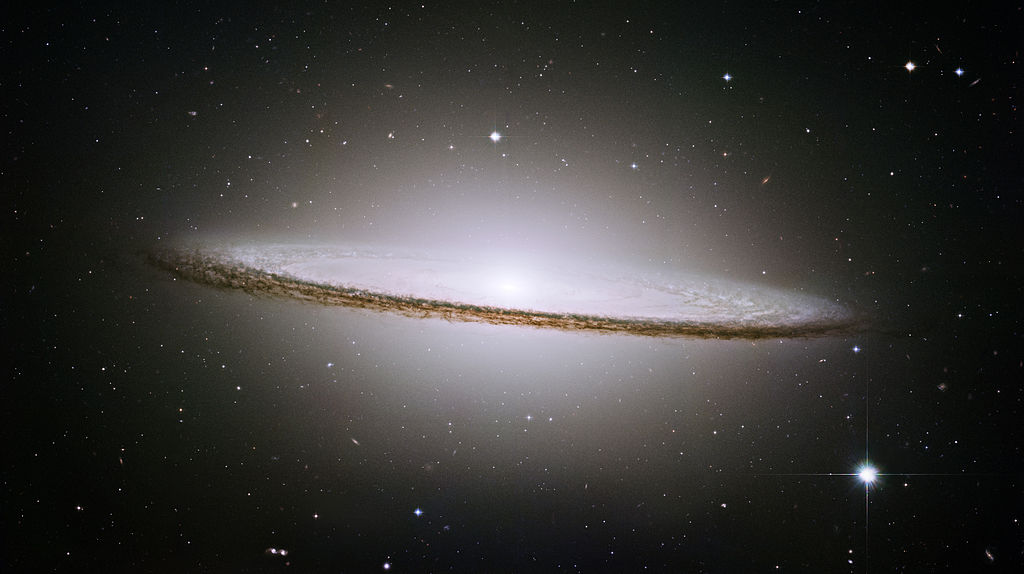
\includegraphics[height=5cm]{sombrero.jpg}
\end{frame}

\begin{frame}
  \center
  \frametitle{Branches of physics by research}
  \includegraphics[height=5cm]{m87.jpg}
\end{frame}

\begin{frame}
  \center
  \frametitle{Branches of physics by research}
  \includegraphics[height=5cm]{eht.jpg}
\end{frame}

\begin{frame}
  \center
  \frametitle{Branches of physics by research}
  \includegraphics[height=5cm]{hl_bh.jpg}
\end{frame}

\begin{frame}
  \center
  \frametitle{Branches of physics by research}
  \includegraphics[height=5cm]{gargantua.jpg}
\end{frame}

\begin{frame}
  \center
  \frametitle{Branches of physics by research}
  \includegraphics[height=5cm]{lensing.jpg}
\end{frame}

\begin{frame}
  \center
  \frametitle{Branches of physics by research}
  \includegraphics[height=5cm]{deep.jpg}
\end{frame}

\begin{frame}
  \center
  \frametitle{Branches of physics by research}
  \includegraphics[height=5cm]{cmb.jpg}
\end{frame}

\begin{frame}
  \center
  \frametitle{Branches of physics by research}
  \includegraphics[height=5cm]{big_bang.jpg}
\end{frame}

\begin{frame}
  \frametitle{Open problems}
  \begin{itemize}
    \item<1-> Some \textbf{general problems} (I know nothing about these!):
      \begin{itemize}
	\item<2-> We don't know how to interpret quantum mechanics
	\item<3-> We don't have a grand unified theory (or if the standard model is complete)
	\item<4-> Why does time flow forward, is this an artefact of consciousness, is causality ever violated?
	\item<5-> We don't know where the dimensionless physical constants come from
      \end{itemize}
  \end{itemize}
\end{frame}

\begin{frame}
  \frametitle{Open problems}
  \begin{itemize}
    \item<1-> Some \textbf{gravitational} and \textbf{cosmological} problems:
      \begin{itemize}
	\item<2-> We don't have a quantum theory of gravity
	\item<3-> We don't know what dark matter is
	\item<4-> We don't know what dark energy is
	\item<5-> We don't know if the universe is finite, infinite or superinfinite
	\item<6-> We don't know why the universe is so flat 
	\item<7-> We don't know for sure if the big bang even happened
      \end{itemize}
  \end{itemize}
\end{frame}

\begin{frame}
  \frametitle{Some things we will need\ldots}
  \begin{itemize}
    \item<1-> As we said earlier, \textbf{physics} is a fundamental part of the \textbf{mathematical description of the world}
    \item<2-> We therefore need to introduce some maths to make any progress whatever:
      \begin{itemize}
	\item<3-> Calculus
	\item<4-> Differential equations
	\item<5-> Linear algebra
	\item<6-> Differential geometry 
      \end{itemize}
    \item<7-> In the UK this material is usually taught to ages 17-22, so \textbf{don't take it too seriously}!
    \item<8-> Idea is to give a \textbf{basic exposure} to these ideas
  \end{itemize}
\end{frame}

\begin{frame}
  \frametitle{Calculus}
  \textit{[A quip] that the physicist Richard Feynman made to the novelist Herman Wouk when they were discussing the Manhattan Project. Wouk was doing research for a big novel he hoped to write about World War II, and he went to Caltech to interview physicists who had worked on the bomb, one of whom was Feynman. After the interview, as they were parting, Feynman asked Wouk if he knew calculus. No, Wouk admitted, he didn’t. “You had better learn it,” said Feynman. “It’s the language God talks.”}
\end{frame}

\begin{frame}
  \frametitle{Calculus}
  \begin{itemize}
    \item<1-> Begin with a function, $y=f(x)$, basic statement of one variable depending on another
    \item<2-> Define the \textbf{derivative} of $y$ with respect to $x$
      <3->\begin{equation*}
	\frac{\mathrm{d}y}{\mathrm{d}x}=\lim_{\delta x\to 0}\frac{f(x+\delta x)-f(x)}{\delta x}
	\label{<+label+>}
      \end{equation*}
    \item<4-> This is a purely \textbf{formal} definition
    \item<5-> Don't get too hung up on what \textbf{differentials} $\mathrm{d}y$ and $\mathrm{d}x$ mean!
    \item<6-> Interpet it as the \textbf{rate of change} of $y$ with respect to $x$
  \end{itemize}
\end{frame}

\begin{frame}
  \frametitle{Calculus}
  \begin{itemize}
    \item<1-> Properties of differentiation:
      \begin{itemize}
	\item<2-> \textbf{Linearity}
	\item<3-> \textbf{Leibniz rule}
	\item<4-> \textbf{Chain rule}
      \end{itemize}
  \end{itemize}
\end{frame}

\begin{frame}
  \frametitle{Calculus}
  \begin{itemize}
    \item<1-> Simplest example, polynomial function:
      \begin{equation*}
	f(x)=c_0+c_1x+c_2x^2+c_3x^3+\cdots
	\label{<+label+>}
      \end{equation*}
    \item<2-> Take any term and apply the formula for differentiation:
      \begin{equation*}
	\frac{\mathrm{d}c_nx^n}{\mathrm{d}x}=\lim_{\delta x\to 0}\frac{c_n(x+\delta x)^n-c_nx^n}{\delta x}
      \end{equation*}
    \item<3-> Easy to then find derivatives of any polynomial by using the linearity property
  \end{itemize}
\end{frame}

\begin{frame}
  \frametitle{Calculus}
  \begin{itemize}
    \item<1-> The inverse operation is called \textbf{integration} and write it this way
      \begin{equation*}
	g(x)=\frac{\mathrm{d}f(x)}{\mathrm{d}x}\implies f(x)=\int g(x)\mathrm{d}x
	\label{<+label+>}
      \end{equation*}
    \item<2-> We have a formula to go from a function to its derivative, but \textbf{not} the other way around
    \item<3-> The only way to proceed is to \textbf{notice} that if $f(x)$ differentiates to $g(x)$, then it must be the correct answer!
  \end{itemize}
\end{frame}

\begin{frame}
  \frametitle{Calculus}
  \begin{itemize}
    \item<1-> Simplest example is to stick to polynomials and find f(x) such that:
      \begin{equation*}
	g(x)=4x^3, \quad f(x)=\int g(x)\mathrm{d}x
	\label{<+label+>}
      \end{equation*}
    \item<2-> We find
\begin{equation}
  f(x)=x^4+c
  \label{<+label+>}
\end{equation}
    \item<3-> The $+c$ part encodes the information lost in the process of differentiation, and we can see this from a discussion of \textbf{area under a curve}
  \end{itemize}
\end{frame}

\begin{frame}
  \frametitle{Calculus}
  \begin{itemize}
    \item<1-> Time to introduce a pair of very important functions
      \begin{equation*}
	\sin(x), \quad \cos(x)
      \end{equation*}
    \item<2-> These are the \textbf{trigonometric} functions
    \item<3-> Someone probably told you these have something to do with \textbf{triangles}, which is true but not so important in physics
    \item<4-> Equivalently, someone might have told you that these functions have something to do with waves, which is also not exactly wrong\ldots
  \end{itemize}
\end{frame}

\begin{frame}
  \frametitle{Calculus}
  \begin{itemize}
    \item<1-> Let's start with $\sin(x)$, we can see precisely what it is doing to $x$ by introducing the notion of a \textbf{power series}:
      \begin{equation*}
	\sin(x)=\sum_{n=0}^{\infty}\frac{(-1)^nx^{2n+1}}{(2n+1)!}
      \end{equation*}
    \item<2-> Don't be too concerned with this sigma and factorial notation, it translates to something very like a polynomial:
      \begin{equation*}
	\sin(x)=x-\frac{1}{6}x^3+\frac{1}{120}x^5-\frac{1}{5040}x^7+\cdots
	\label{<+label+>}
      \end{equation*}
    \end{itemize}
\end{frame}

\begin{frame}
  \frametitle{Calculus}
  \begin{itemize}
    \item<1-> Should be able to find the derivative of $\sin(x)$ quite easily, just apply the rules:
      \begin{equation*}
	\frac{\mathrm{d}\sin(x)}{\mathrm{d}x}=\sum_{n=0}^{\infty}\frac{(-1)^nx^{2n}}{(2n)!}
	\label{<+label+>}
      \end{equation*}
    \item<2-> By differentiating $\sin(x)$ we've stumbled on the definition of $\cos(x)$, what happens if we keep differentiating?
  \end{itemize}
\end{frame}

\begin{frame}
  \frametitle{Calculus}
  \begin{itemize}
    \item<1-> The \textbf{trigonometric} functions are how we rotate points in \textbf{three-dimensional space} (hence their application in triangles), we will touch on how to do this later, but $x$ just becomes the  \textbf{angle} of rotation
    \item<2-> There is another very similar pair of functions:
      \begin{equation*}
	\sinh(x), \quad \cosh(x)
      \end{equation*}
    \item<3-> These are known as the \textbf{hyperbolic} functions, they are used in the rotation of \textbf{four-dimensional space-time}
  \end{itemize}
\end{frame}

\begin{frame}
  \frametitle{Calculus}
  \begin{itemize}
    \item<1-> The \textbf{power series} for $\sinh(x)$ is as follows:
      \begin{equation*}
	\sinh(x)=\sum_{n=0}^{\infty}\frac{x^{2n+1}}{(2n+1)!}
	\label{<+label+>}
      \end{equation*}
    \item<2-> Once again a simple differentiation is sufficient to obtain $\cosh(x)$:
      \begin{equation*}
	\cosh(x)=\sum_{n=0}^{\infty}\frac{x^{2n}}{(2n)!}
	\label{<+label+>}
      \end{equation*}
    \item<3-> And this process continues in an obvious manner\ldots
  \end{itemize}
\end{frame}

\begin{frame}
  \frametitle{Calculus}
  \begin{itemize}
    \item<1-> The trigonometric and hyperbolic functions clearly have very similar power series and must be related
    \item<2-> To see how, we will need the \textbf{exponential} function:
      \begin{equation*}
	e^x
      \end{equation*}
    \item<3-> The number $e\approx 2.71828$ is known as \textbf{Euler's constant} -- this particular value enables us to write the following power series:
      \begin{equation*}
	e^x=\sum_{n=0}^{\infty}\frac{x^n}{n!}
      \end{equation*}
  \end{itemize}
\end{frame}

\begin{frame}
  \frametitle{Calculus}
  \begin{itemize}
    \item<1-> Now once again we want to differentiate this function to see what it gives:
      \begin{equation*}
	\frac{\mathrm{d}e^x}{\mathrm{d}x}=e^x
      \end{equation*}
    \item<2-> As with the trigonometric and hyperbolic functions, the exponential function emerges in all areas of physics, you have probably heard already that it describes \textbf{radioactive decay}, but also e.g. the behaviour of the size of the universe near its beginning (\textbf{inflation}) and end (\textbf{de-Sitter expansion})
  \end{itemize}
\end{frame}

\begin{frame}
  \frametitle{Calculus}
  \begin{itemize}
    \item<1-> The relation between the \textbf{exponential} and \textbf{hyperbolic} functions is fairly clear from the power series, we just need to get to grips with \textbf{even} and \textbf{odd} functions:
      \begin{equation}
	\sinh(x)=\frac{1}{2}\left( e^x-e^{-x} \right), \quad \cosh(x)=\frac{1}{2}\left( e^x+e^{-x} \right)
	\label{<+label+>}
      \end{equation}
    \item<2-> An obvious consequence of this is (known in mathematics as a \textbf{corollary}):
      \begin{equation*}
	e^x=\sinh(x)+\cosh(x)	
      \end{equation*}
    \item<3-> And another less obvious corollary:
      \begin{equation*}
	\cosh^2(x)-\sinh^2(x)=1
      \end{equation*}
  \end{itemize}
\end{frame}

\begin{frame}
  \frametitle{Calculus}
  \begin{itemize}
    \item<1-> The case of the \textbf{exponential} and \textbf{trigonometric} functions is a bit harder, we need to include \textbf{imaginary numbers} to account for all those strange $-1$ factors in the power series:
      \begin{equation*}
	i^2=-1
      \end{equation*}
    \item<2-> The only place we really unavoidably need imaginary (or \textbf{complex}) numbers is in \textbf{quantum mechanics} and its special-relativistic generalisation, \textbf{quantum field theory}
    \item<3-> However, keep in mind that physics only works because some fundamental quantities (i.e. \textbf{wavefunctions}) that describe real phenomena, can't be expressed using real numbers
  \end{itemize}
\end{frame}

\begin{frame}
  \frametitle{Calculus}
  \begin{itemize}
    \item<1-> We find:
      \begin{equation*}
	\sin(x)=\frac{1}{2i}\left( e^{ix}-e^{-ix} \right), \quad \cos(x)=\frac{1}{2}\left( e^{ix}+e^{-ix} \right)
      \end{equation*}
    \item<2-> Again there is a neat corollary to this:
      \begin{equation*}
	e^{ix}=\cos(x)+i\sin(x)
      \end{equation*}
    \item<3-> And something you have probably met before:
      \begin{equation*}
	\cos^2(x)+\sin^2(x)=1
      \end{equation*}
  \end{itemize}
\end{frame}

\begin{frame}
  \frametitle{Calculus}
  \begin{itemize}
    \item<1-> Before we move on to some physics, try differentiating the following:
      \begin{itemize}
	\item<2-> $x^2+5x^3+8$
	\item<3-> $\left( 3x^3+8x^8 \right)e^x$
	\item<4-> $\sin(x)\cos(x)$
	\item<5-> $\sin^2(x)\cos^2(x)$
      \end{itemize}
    \item<6-> Next, try these integrals:
      \begin{itemize}
	\item<7-> $\int \sin(x)\mathrm{d}x$
	\item<8-> $\int e^x\left( \sin(x)+\cos(x) \right)\mathrm{d}x$
	\item<9-> $\int x^5\left( \cosh(x)+\frac{1}{6}x\sinh(x) \right)\mathrm{d}x$
	\item<10> $\int e^{-x}\mathrm{d}x$
      \end{itemize}
  \end{itemize}
\end{frame}

\begin{frame}
  \frametitle{Calculus}
  \begin{itemize}
    \item<1-> Now apply the Leibniz and chain rules carefully when differentiating these:
      \begin{itemize}
	\item<2-> $\frac{x^2+5x^3+8}{\sin^2(x)\cos^2(x)}$
	\item<3-> $\cosh(\sin(e^{2x}))$
	\item<4-> $\sin(x+1)$
      \end{itemize}
  \end{itemize}
\end{frame}

\begin{frame}
  \frametitle{Differential equations}
  \begin{itemize}
    \item<1-> Now we've introduced \textbf{calculus}, we have a very powerful kit of tools for describing physical phenomena: any sensible description of the world must include some notion of rates of change (derivatives) and accumulations of one function over some variable (integrals)
    \item<2-> Almost all \textbf{physical laws} need to be cast in the language of calculus to hold any meaning
    \item<3-> Almost all physical laws are expressed in terms of \textbf{differential equations}
    \item<4-> However they are often expressed simply as \textbf{equations} instead:
      \begin{equation*}
	F=\frac{Gm_1m_2}{r^2}
      \end{equation*}
  \end{itemize}
\end{frame}

\begin{frame}
  \frametitle{Differential equations}
  \begin{itemize}
    \item<1-> Differential equations are just equations which contain derivatives of a function
    \item<2-> An equation:
      \begin{equation*}
	\frac{f(x)}{x^2}=-\lambda^2 f(x)
      \end{equation*}
    \item<3-> Clearly this just solves to $f(x)=0$, for general $x$ and $\lambda$: not very exciting!
    \item<4-> A more interesting differential equation:
      \begin{equation*}
	\frac{\mathrm{d}^2f(x)}{\mathrm{d}x^2}=-\lambda^2f(x)
      \end{equation*}
  \end{itemize}
\end{frame}

\begin{frame}
  \frametitle{Differential equations}
  \begin{itemize}
    \item<1-> It is likely you will mostly meet \textbf{linear} differential equations in school and furthermore that these re \textbf{ordinary} differential equations (ODEs), these take the general form:
      \begin{equation*}
	\sum_{n=0}^{\infty}c_n\frac{\mathrm{d}^nf(x)}{\mathrm{d}x^n}=g(x)
      \end{equation*}
    \item<2-> Linear ODEs can be further divided into \textbf{homogeneous} and \textbf{inhomogeneous} depending on whether $g(x)$ is present\ldots
    \item<3-> Luckily, linear ODEs are incredably important in basic physics, and we already have most of the tools we need to solve them!
  \end{itemize}
\end{frame}

\begin{frame}
  \frametitle{Differential equations}
  \begin{itemize}
    \item<1-> Linear ODEs are always solved to some extent by the exponential function
    \item<2-> To see this, consider a very simple example of a circuit with a capacitor and resistor
    \item<3-> We have $V_R=-IR$ and $V_C=\frac{Q}{C}$, but also $\dot{Q}=-I$
    \item<4-> Resultant ODE:
      \begin{equation*}
	\dot{Q}=-\frac{1}{RC}Q	
      \end{equation*}
    \item<5-> So applying what we learned earlier, we have \textbf{exponential decay}:
      \begin{equation*}
	Q=Q_0e^{-\frac{t}{RC}}
      \end{equation*}
  \end{itemize}
\end{frame}

\begin{frame}
  \frametitle{Differential equations}
  \begin{itemize}
    \item<1-> The linear ODE we met at the beginning is known as the \textbf{harmonic oscillator}, it emerges \textbf{all over} physics
    \item<2-> Essence of the problem is that the \textbf{acceleration} of a quantity (rate of change of rate of change) is proportional to that quantity, and tends to act \textbf{against} its motion
    \item<3-> Let's do this from the point of view of circuits again, replace the resistor with an \textbf{inductor}, $V_L=L\dot{I}$
    \item<4-> Should end up with the following:
      \begin{equation*}
	\ddot{Q}=-\frac{1}{LC}Q 
      \end{equation*}
  \end{itemize}
\end{frame}

\begin{frame}
  \frametitle{Differential equations}
  \begin{itemize}
    \item<1-> To solve the harmonic oscillator (also known as \textbf{the simple harmonic equation}), it is helpful to use the linearity property of the ODE
    \item<2-> Should get something like:
      \begin{equation*}
	Q=Q_1\sin\left(\frac{t}{\sqrt{LC}}\right)+Q_2\cos\left(\frac{t}{\sqrt{LC}}\right)
	\label{<+label+>}
      \end{equation*}
    \item<3-> Note that in general, the coefficient at the front occurs because of the linearity of the ODE, since this ODE is of \textbf{2nd order}, we get two constants, i.e. information about $Q$ was lost twice when setting up the system
  \end{itemize}
\end{frame}

\begin{frame}
  \frametitle{Differential equations}
  \begin{itemize}
    \item<1-> When we put the resistor back in what do we find?
  \end{itemize}
\end{frame}

\begin{frame}
  \frametitle{Differential equations}
  \begin{itemize}
    \item<1-> What we've been looking at so far regarding circuits is actually a \textbf{coupled} ODE system, there were two unknown functions: $Q(t)$, $I(t)$
    \item<2-> Since we were able to eliminate $I(t)$ from the system in a trivial way, we only had to solve one ODE
  \end{itemize}
\end{frame}

\begin{frame}
  \frametitle{Differential equations}
  \begin{itemize}
    \item<1-> Consider the following example from ecology. The number of foxes is $f(t)$, and the number of rabbits is $r(t)$ and the populations change according to the following rules:
      \begin{itemize}
	\item<2-> Rabbits live forever\ldots unless they are eaten by foxes
	\item<3-> Rabbits never reproduce\ldots
	\item<4-> Foxes live forever\ldots
	\item<5-> Foxes don't reproduce either, but they do eat rabbits
	\item<6-> The rate at which foxes eat rabbits is proportional to the number of foxes and the number of rabbits
      \end{itemize}
  \end{itemize}
\end{frame}

\begin{frame}
  \frametitle{Differential equations}
  \begin{itemize}
    \item<1-> Now add the following feature:
      \begin{itemize}
	\item<2-> Foxes get to reproduce, but only at a rate proportional to their rabbit-eating
      \end{itemize}
  \end{itemize}
\end{frame}

\begin{frame}
  \frametitle{Differential equations}
  \begin{itemize}
    \item<1-> Lastly:
      \begin{itemize}
	\item<2-> Foxes die naturally and at a rate proportional to their population
	\item<3-> Rabbits reproduce like foxes do, i.e. by eating -- in this case they eat at a rate proportional to their own population size (i.e. their food source is not constrained)
      \end{itemize}
  \end{itemize}
\end{frame}

\begin{frame}
  \frametitle{Differential equations}
  \begin{itemize}
    \item<1-> The full system of relations results in the \textbf{Lotka-Volterra} equations, these can't generally be solved cleanly but we can get an idea through \textbf{numerical ODE techniques} of how things play out\ldots
    \item<2-> They also apparently have some applications in physics\ldots
  \end{itemize}
\end{frame}

\begin{frame}
  \frametitle{Differential equations}
  \textit{Energy transport and confinement in tokamak fusion plasmas is usually determined by the coupled nonlinear interactions of small-scale drift turbulence and larger scale coherent nonlinear structures, such as zonal flows, together with free energy sources such as temperature gradients. Zero-dimensional models, designed to embody plausible physical narratives for these interactions, can help to identify the origin of enhanced energy confinement and of transitions between confinement regimes. A prime zero-dimensional paradigm is predator-prey or \textbf{Lotka-Volterra}. Here, we extend a successful three-variable (temperature gradient; microturbulence level; one class of coherent structure) model in this genre [M. A. Malkov and P. H. Diamond, Phys. Plasmas 16, 012504 (2009)], by adding a fourth variable representing a second class of  \ldots}
\end{frame}

\begin{frame}
  \frametitle{Differential equations}
  \begin{itemize}
    \item<1-> So far we've been wrapped up with ODEs
    \item<2-> Unfortunately most of the really interesting differential equations in physics are \textbf{partial} differential eqations (PDEs)
    \item<3-> These sound a lot worse than they are, but before we look at them we need to understand partial differentiation
    \item<4-> We can easily think of a function of \textbf{two or more variables}, e.g. $f(x,y)$:
      \begin{equation*}
	f(x,y)=\cosh(x)+3xy-\sin(y)
      \end{equation*}
  \end{itemize}
\end{frame}

\begin{frame}
  \frametitle{Differential equations}
  \begin{itemize}
    \item<1-> Partial differentiation is nothing more than differentiation with respect to a particular variable, it really is that simple!
      \begin{equation*}
	f(x,y)=\cosh(x)+3xy-\sin(y)
      \end{equation*}
    \item<2-> So for this function we have
      \begin{equation*}
	\frac{\partial f(x,y)}{\partial x}=\sinh(x)+3y, \quad \frac{\partial f(x,y)}{\partial y}=3x-\cos(y)
	\label{<+label+>}
      \end{equation*}
    \item<3-> The only subtlety is the use of $\partial$ instead of $\mathrm{d}$\ldots they mean \textbf{exactly the same thing}
  \end{itemize}
\end{frame}

\begin{frame}
  \frametitle{Differential equations}
  \begin{itemize}
    \item<1-> Before we get to check out some more physics, try the following examples:
      \begin{itemize}
	\item<2-> $y\frac{\partial (xy)}{\partial x}-x\frac{\partial (xy)}{\partial y}$
	\item<3-> $\frac{\partial^2 \cosh(x^2+y^2)}{\partial x\partial y}$
      \end{itemize}
  \end{itemize}
\end{frame}

\begin{frame}
  \frametitle{Differential equations}
  \begin{itemize}
    \item<1-> Very often in physics we are dealing with a problem in which a quantity varies simultaneously in \textbf{space} and \textbf{time}
    \item<2-> This is different to the simpler problem in which position depends on time, i.e. classical mechanics (see Seminar 3)
    \item<3-> For example, we might have temperature $T$ of air depending simultaneously on time, $t$, and the position in a room, which we can describe by $x$, $y$, and $z$ -- this means our equations will involve $T(t,x,y,z)$
    \item<4-> Generally this sort of thing comes up in \textbf{field theories}, such theories have dominated fundamental physics for the last 100 years!
  \end{itemize}
\end{frame}

\begin{frame}
  \frametitle{Differential equations}
  \begin{itemize}
    \item<1-> Most field theories end up producing some kind of \textbf{wave equation}, temperature does \texbf{not} form waves (for reasons you may come across in Week 2)
    \item<2-> For example pressure, $P(t,x,y,z)$, and the electromagnetic fields $\mathbf{E}(t,x,y,z)$ and $\mathbf{B}(t,x,y,z)$, although the last two are \textbf{vector} fields
  \end{itemize}
\end{frame}

\begin{frame}
  \frametitle{Differential equations}
  \begin{itemize}
    \item<1-> To see why the wave equation predicts waves, consider an example in one space dimension
    \item<2-> A string has tension $\tau$ and mass per unit length $\mu$, it is extended between two points which are spatially separated down $x$, and its deviation from a straight line at any point $x$ and time $t$ is given by $f(t,x)$
    \item<3-> To see how the string behaves, we will need a careful application of Newton's three laws and some trigonometry (perhaps we will get there in Seminar 3)
  \end{itemize}
\end{frame}

\begin{frame}
  \frametitle{Differential equations}
  \begin{itemize}
    \item<1-> The result, however, is the following wave equation:
      \begin{equation*}
	\mu\frac{\partial^2f(t,x)}{\partial t^2}=\tau\frac{\partial^2f(t,x)}{\partial x^2}
      \end{equation*}
    \item<2-> This looks a bit formidable, but notice that it is solved by the following:
      \begin{equation*}
	f(t,x)=\sin\left(x-\sqrt{\frac{\tau}{\mu}}t\right), \quad f(t,x)=\sin\left(x+\sqrt{\frac{\tau}{\mu}}t\right)
      \end{equation*}
    \item<3-> Think about what these functions actually mean, we have a $\sin$-wave moving with speed $v=\sqrt{\tau/\mu}$ along the string
  \end{itemize}
\end{frame}

\begin{frame}
  \frametitle{Differential equations}
  \begin{itemize}
    \item<1-> In fact, there is nothing special about our choice of $\sin$ function, the \textbf{shape} of the wave is completely irrelevent, all that matters is that it moves along the string in \textbf{either} direction at speed $v$
    \item<2-> The wave equation for waves on a string is an example of a \textbf{field theory} in time and one spatial dimension, it isn't an expecially fundamental field theory because it relies on non-relativistic notions of mass and acceleration
    \item<3-> A very similar theory applies to gases, and results in the \textbf{acoustic wave equation},
      \begin{equation*}
	v^2\frac{\partial^2P(t,x,y,z)}{\partial t^2}=\frac{\partial^2P(t,x,y,z)}{\partial x^2}+\frac{\partial^2P(t,x,y,z)}{\partial y^2}+\frac{\partial^2P(t,x,y,z)}{\partial z^2}
      \end{equation*}
  \end{itemize}
\end{frame}

\begin{frame}
  \frametitle{Differential equations}
  \begin{itemize}
    \item<1-> The sound speed is given by the dependence of the pressure $P$ on the density $\rho$, but the details of \textbf{why} will have to wait for Week 2
      \begin{equation*}
	v^2=\frac{\mathrm{d}P}{\mathrm{d}\rho}
      \end{equation*}
    \item<2-> The resulting equation looks formidable because we have \textbf{three} spatial dimensions, but by some guess-work we can find a simple solution
      \begin{equation*}
	v^2\frac{\partial^2P(t,x,y,z)}{\partial t^2}=\frac{\partial^2P(t,x,y,z)}{\partial x^2}+\frac{\partial^2P(t,x,y,z)}{\partial y^2}+\frac{\partial^2P(t,x,y,z)}{\partial z^2}
      \end{equation*}
    \item<3-> \textbf{plane waves} of the simple form $P(t,x,y,z)=f(x-vt))$, i.e. moving at speed $v$ down the $x$ direction
  \end{itemize}
\end{frame}

\begin{frame}
  \frametitle{Differential equations}
  \begin{itemize}
    \item<1-> So we have seen that the wave equation takes a predictable form in these theories, only the \textbf{speed} of the waves changes due to the details of the \textbf{theory}
    \item<2-> In Seminar 4 we may be able to talk about the \textbf{Maxwell equations}, these are the four equations which govern the elextromagnetic fields, (obviously a \textbf{field theory}), and two of them constitute a \textbf{coupled} wave equation
    \item<3-> The result is that these fields can move on their own through space (i.e. without any charges or currents) at a speed known as $c$, the \textbf{speed of light}
  \end{itemize}
\end{frame}

\begin{frame}
  \frametitle{Differential equations}
  \begin{itemize}
    \item<1-> It doesn't stop there: just as we have a fundamental theory for electromagnetism, the wave equation with $v=c$ also emerges in the most famous theory of \textbf{gravity}, i.e. \textbf{general relativity} -- this gives rise to \textbf{gravity waves}
    \item<2-> The wave equation has a cousin, known as the \textbf{diffusion equation}, e.g. for temperature in one spatial dimension:
      \begin{equation*}
	\frac{\partial T(t,x)}{\partial t}=D\frac{\partial^2 T(t,x)}{\partial x^2}
      \end{equation*}
  \end{itemize}
\end{frame}

\begin{frame}
  \frametitle{Differential equations}
  \begin{itemize}
    \item<1-> We mentioned before that heat (or temperature) tends not to form waves, but the diffusion equation can give \textbf{wave-like behaviour} if we make time \textbf{imaginary}:
      \begin{equation*}
	i\frac{\partial\Psi(t,x)}{\partial t}=-\frac{\hbar}{2m}\frac{\partial^2\Psi(t,x)}{\partial x^2}	
      \end{equation*}
    \item<2-> This is the \textbf{Schr\"odinger equation}, and it describes the behaviour of the \textbf{wavefunction} $\Psi(t,x)$ in one dimension, the fundamental description of a particle in quantum mechanics
  \end{itemize}
\end{frame}

\end{document}


